\subsection{Transformer \& Models Used}

The transformer architecture used in the natural language processing (NLP) field is a revolutionary technology. By replacing traditional recurrent and convolutional layers with a mechanism based on self-attention \cite{vaswani_attention_2023}, it enables the model can capture the contextual 
relationships more effectively than previous architectures.

\subsection{BERT \& GPT-2}

The models we will use in this study are two popular transformer-based models, BERT (Bidirectional Encoder Representations from Transformers) and GPT (Generative Pre-trained Transformer), they are two distinct models with different component stacks, and they are designed with different approaches. BERT \cite{koroteev_bert_2021} is an encoder-only model based on a bidirectional deep learning model and can capture the information from both directions, making it suitable to understand language structure and can handle tasks like question answering, named entity recognition etc.
In contrast, GPT and its new versions (GPT-2, GPT-3, and GPT-4) are decoder-only models; they focus on an auto-regressive approach \cite{zhao_survey_2025}, and its token is based on a left-to-right manner, which makes it more suitable to generate creative content.

\begin{figure*}[t]
    \centering
    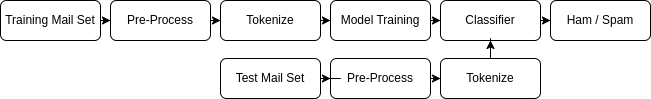
\includegraphics[width=1\linewidth]{figure/mail_classification_process.png} \hfill
    \caption{Spam email classification process}
    \label{fig:spam-email-classification-process}
\end{figure*}

\subsection{Evaluation Metrics}

We will use the commonly used accuracy, precision, recall, and F1-Score as evaluation indicators on the test set, which can provide clear and interpretable metrics for assessing classification performance, we will also compare train loss and test loss to find the most suitable epoch number.
